% ><>< ================================================================= ><>< %
% ><><     scoup:- Simulate Codon Sequences with Darwinian Selection     ><>< %
% ><><           Incorporated as an Ornstein-Uhlenbeck Process           ><>< %
% ><><                       ~~~~~~~~~~~~~~~~~~~~~                       ><>< %
% ><><                          13th June 2025.                          ><>< %
% ><>< ================================================================= ><>< %

\documentclass[12pt]{article}

% ><><                      Load necessary packages                      ><>< %
\usepackage{tikz}
\usepackage{pifont}
\usepackage{multirow}
\usepackage{enumerate}
\usepackage{graphicx, color}
\usepackage[hidelinks]{hyperref}
\usepackage{amsmath, amsthm, amsfonts, amssymb}
\DeclareMathAlphabet{\mathpzc}{OT1}{pzc}{m}{it}
\usepackage[paperheight=4.28in, paperwidth=10.4in,%10.9in,
    margin=.1in, heightrounded]{geometry}
 \renewcommand{\familydefault}{\sfdefault}
% --------------------------------------------------------------------------- %

% ><><                          Define colours                           ><>< %
\definecolor{d00}{rgb}{0.00, 0.00, 0.00}
\definecolor{d02}{rgb}{0.80, 0.80, 0.80}
\definecolor{d03}{rgb}{0.13, 0.55, 0.13}
\definecolor{d04}{rgb}{0.50, 0.50, 0.50}
\definecolor{d05}{rgb}{1.00, 1.00, 1.00}
% --------------------------------------------------------------------------- %

% ><><                      Tikz shapes and designs                      ><>< %
\usetikzlibrary{positioning}
\usetikzlibrary{shapes, arrows}
\usetikzlibrary{shapes.gates.logic.US}
\usetikzlibrary{decorations.pathreplacing}
\usetikzlibrary{decorations.pathmorphing,patterns}
\usetikzlibrary{calc, patterns, decorations.markings}

% ><>< ==== ><>< % Lines
\tikzstyle{Line} = [draw, line width=.12cm, rounded corners, -latex']
% ><>< ==== ><>< % Rectangles
\tikzstyle{arect} = [draw, rectangle, minimum width=-0.7em,
    minimum height=2em, text centered, rounded corners,
    fill=white, line width=.08cm]
% ><>< ==== ><>< % Gate
\tikzstyle{on}=[draw, chamfered rectangle,
    white, fill=d03, double=d03, very thick,
    text width=4em, minimum height=3em, text centered, line width=.08cm]
\tikzstyle{off}=[draw, chamfered rectangle,
    white, fill=red, double=red, very thick,
    text width=4em, minimum height=3em, text centered, line width=.08cm]
\tikzstyle{elpz} = [draw, ellipse, line width=.1cm]
% ><>< ==== ><>< % Tape
\tikzstyle{dcmt} = [draw, tape, minimum width=6cm,
    d00, tape bend height=0.4cm, minimum height=2em,
    text centered, fill=white, tape bend top = none, line width=.08cm]
% ><>< ==== ><>< % Trapezoid
\tikzstyle{traped} = [draw, trapezium, minimum width=-5em, d00,
    trapezium left angle=97, trapezium right angle=83,
    minimum height=2em, text centered, fill=white, line width=.08cm]
% ><>< ==== ><>< % Cylinder
\tikzstyle{clnd} = [draw, cylinder, minimum width=-2em,
    shape border rotate = 90, minimum height=2em, text centered,
    d00, cylinder uses custom fill, cylinder end fill = d02,
    aspect=0.143, pattern = crosshatch dots, pattern color = d05,
    line width=.08cm]
% --------------------------------------------------------------------------- %

% ><><                          Bespoke Command                          ><>< %
\newcommand{\slate}[2]{
    \begin{minipage}[!t]{#1 cm} \centering #2 \end{minipage}}
% --------------------------------------------------------------------------- %

% ><><                         Begin compilation                         ><>< %
\begin{document}
\thispagestyle{empty}
% --------------------------------------------------------------------------- %
   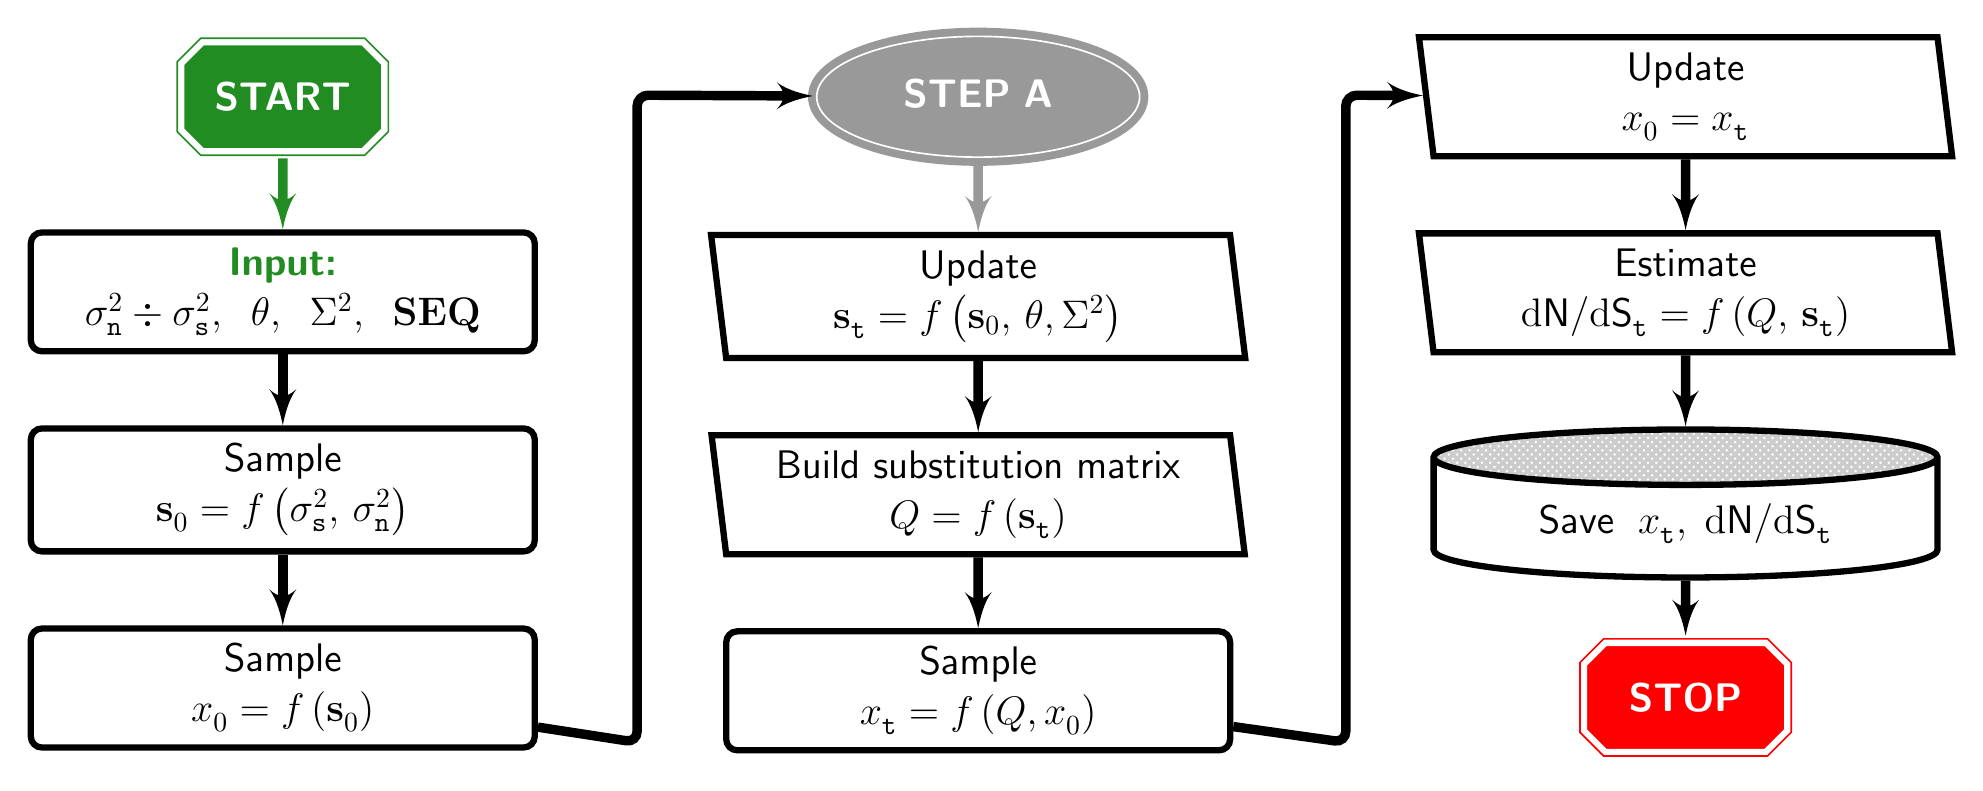
\begin{tikzpicture}[auto, inner sep=2mm, node distance=.9cm]
     \Large
     % ><>< =================== ><>< %
     % ><><     Place nodes     ><>< %
     % ><>< =================== ><>< %
     % \draw [help lines] (-13,-5.1) grid (13,5.1);
     % ><>< =================== ><>< %
     \node [on] (step00) at (-9.0,4.1) {\bf START};
     \node [arect, below=of step00] (step01)
        {\slate{6}{{\color{d03}\textbf{Input:}}\\$\sigma^{2}_{\texttt{n}}
         \div \sigma^{2}_{\texttt{s}},\;\;\theta,\;\;\Sigma^{2}_{},\;\;
         \mathbf{SEQ}$}};
     \node [arect, below=of step01] (step02)
        {\slate{6}{Sample\\$\mathbf{s}_{0}^{}=f\left(\sigma^{2}_{\texttt{s}},
         \,\sigma^{2}_{\texttt{n}}\right)$}};
     \node [arect, below=of step02] (step03)
        {\slate{6}{Sample\\$x_{0}^{}=f\left(\mathbf{s}_{0}^{}\right)$}};
     \node [elpz, text width=2.5cm, text height=1.08em, right=of step00,
        fill=white, double=white, d04!80, xshift=4.45cm] (step04)
        {\slate{2.5}{\color{white}\textbf{STEP A}\vspace*{.2cm}}};
     \node [traped, below=of step04] (step05)
        {\slate{6}{Update \\ $\mathbf{s}_{\texttt{t}}^{}=
         f\left(\mathbf{s}_{0},\,\theta,\Sigma^{2}_{}\right)$}};
     \node [traped, below=of step05] (step06)
        {\slate{6}{Build substitution matrix \\ $Q=f\left(
         \mathbf{s}_{\texttt{t}}^{}\right)$}};
     \node [arect, below=of step06] (step07)
        {\slate{6}{Sample\\$x_{\texttt{t}}^{}=f\left(Q, x_{0}^{}\right)$}};
     \node [traped, right=of step04, xshift=2.65cm] (step08)
        {\slate{6}{Update \\ $x_{0}^{} = x_{\texttt{t}}^{}$}};
     \node [traped, below=of step08] (step09)
        {\slate{6}{Estimate \\ $\mathrm{d}\textsf{N}/
         \mathrm{d}\textsf{S}_{\texttt{t}}^{} =
         f\left(Q,\,\mathbf{s}_{\texttt{t}}^{}\right)$}};
     \node [clnd, aspect=0.11, below=of step09] (step10)
         {\slate{6}{Save\; $x_{\texttt{t}}^{},\;
          \mathrm{d}\textsf{N}/\mathrm{d}\textsf{S}_{\texttt{t}}^{}$}};
     \node [off, below=of step10, yshift=0.2cm] (step11) {\bf STOP};
     % ><>< =================== ><>< %
     % ><><     Draw lines.     ><>< %
     % ><>< =================== ><>< %
     \path [Line, d03] (step00) -- (step01);
     \path [Line] (step01) -- (step02);
     \path [Line] (step02) -- (step03);
     \path [Line] (step03) -- (-4.5,-4.1) -- (-4.5,4.12) -- (step04);
     \path [Line, d04!80] (step04) -- (step05);
     \path [Line] (step05) -- (step06);
     \path [Line] (step06) -- (step07);
     \path [Line] (step07) -- (4.5,-4.1) -- (4.5,4.12) -- (step08);
     \path [Line] (step08) -- (step09);
     \path [Line] (step09) -- (step10);
     \path [Line] (step10) -- (step11);
  \end{tikzpicture}
% --------------------------------------------------------------------------- %

\end{document}

% ><>< ================================================================= ><>< %
% ><><                        DOCUMENT ENDS HERE.                        ><>< %
% ><>< ================================================================= ><>< %